\section{Cơ sở lý thuyết}
Với sự phát triển không ngừng của công nghệ, việc chuyển đổi thông tin từ tài liệu giấy trở thành dạng điện tử đã trở nên cực kỳ quan trọng đối với doanh nghiệp và cá nhân. Trước đây, việc nhập liệu thủ công từ hóa đơn và tài liệu tương tự tốn rất nhiều thời gian, công sức và có nguy cơ sai sót cao. Tuy nhiên, với sự xuất hiện của công nghệ OCR, quá trình này đã trở nên tự động và hiệu quả hơn, giúp tiết kiệm thời gian và tối ưu hóa quá trình làm việc.

Trong chương này, ta sẽ bắt đầu bằng việc tìm hiểu về cơ bản của công nghệ OCR, một công nghệ quan trọng đã thay đổi cách chúng ta xử lý và quản lý thông tin, khám phá cách OCR có thể phân tích hình ảnh, xác định kí tự và từ, và biến đổi chúng thành dạng văn bản có thể xử lý.

Qua đó, chương cơ sở lý thuyết này sẽ tạo nền tảng kiến thức quan trọng cho việc hiểu rõ hơn về công nghệ OCR và tầm quan trọng của nó trong việc tối ưu hóa quá trình nhận dạng hóa đơn.

\subsection{Nhận dạng ký tự quang học}
\subsubsection{Nhận dạng ký tự quang học là gì?}
Nhận dạng ký tự quang học hay còn gọi là OCR đây là quá trình chuyển đổi một hình ảnh văn bản viết tay, đánh máy hoặc in thành định dạng văn bản mà máy có thể hiểu được. Nó được sử dụng rộng rãi để nhận dạng và tìm kiếm văn bản từ các tài liệu điện tử hoặc để xuất bản văn bản trên một trang web. \cite{aws, survey_ocr_Applications}

OCR được sử dụng rộng rãi như một hình thức nhập dữ liệu từ các bản ghi dữ liệu giấy in - cho dù đó là tài liệu hộ chiếu, hóa đơn, sao kê ngân hàng, biên lai vi tính hóa, danh thiếp, thư, dữ liệu in hoặc bất kỳ tài liệu phù hợp nào - đó là một phương pháp phổ biến để số hóa các văn bản in sao cho chúng có thể được chỉnh sửa, tìm kiếm, lưu trữ bằng điện tử, hiển thị trực tuyến và được sử dụng trong các quy trình máy như điện toán nhận thức, dịch máy, chuyển văn bản thành giọng nói (trích xuất), dữ liệu chính và khai thác văn bản. OCR là một lĩnh vực nghiên cứu về nhận dạng mẫu, trí tuệ nhân tạo và thị giác máy tính.\cite{wiki}

Nhận dạng ký tự quang học đã được áp dụng vào nhiều ứng dụng khác nhau. Dưới đây là một  số ứng dụng của OCR: \cite{survey_ocr_Applications}
\begin{itemize}
    \item \textbf{Nhận dạng chữ viết tay:} Máy tính để nhận và diễn dịch thông tin viết tay rõ ràng từ các nguồn như tài liệu giấy, ảnh, màn hình cảm ứng và các thiết bị khác. Hình ảnh văn bản viết có thể được cảm nhận "ngoại tuyến" từ tờ giấy thông qua quét quang học hoặc nhận dạng từ thông minh. Một cách khác, các chuyển động của đầu bút viết có thể được cảm nhận "trực tuyến", ví dụ như bề mặt màn hình máy tính dựa trên bút viết.
    \item \textbf{Ngân hàng:} Được sử dụng để xử lý séc mà không cần sự tham gia của con người. Một tờ séc có thể được đặt vào máy, trong đó hệ thống quét số tiền cần phát hành và số tiền chính xác sẽ được chuyển khoản. Công nghệ này đã gần như được hoàn thiện cho các séc được in ấn và cũng khá chính xác đối với các séc viết tay, giảm thiểu thời gian chờ đợi tại ngân hàng.
    \item \textbf{Chăm sóc sức khỏe:} Các chuyên gia y tế luôn phải đối mặt với số lượng lớn các biểu mẫu cho mỗi bệnh nhân, bao gồm cả biểu mẫu bảo hiểm cũng như các biểu mẫu sức khỏe chung. Để theo kịp với tất cả thông tin này, việc nhập dữ liệu liên quan vào một cơ sở dữ liệu điện tử có thể được truy cập khi cần thiết. Các công cụ xử lý biểu mẫu, được cung cấp bởi công nghệ OCR, có khả năng trích xuất thông tin từ các biểu mẫu và đưa vào cơ sở dữ liệu, để mỗi dữ liệu bệnh nhân được ghi lại đúng thời điểm.
    \item \textbf{Captcha:} Trong CAPTCHA, một hình ảnh gồm các ký tự hoặc số được tạo ra, bị mờ đi bằng các kỹ thuật biến dạng hình ảnh, biến đổi kích thước và phông chữ, phông nền gây xao lãng, đoạn ngẫu nhiên, đánh dấu và nhiễu trong hình ảnh. Hệ thống này có thể được sử dụng để loại bỏ nhiễu và phân đoạn hình ảnh để làm cho hình ảnh dễ xử lý cho các hệ thống OCR 
    \item \textbf{Ảnh hóa đơn:} Được sử dụng rộng rãi trong nhiều ứng dụng kinh doanh để theo dõi hồ sơ tài chính và ngăn chặn việc tích lũy các khoản thanh toán chồng chất.
    \item \textbf{Nhận dạng biển số xe}: Sử dụng để tự động nhận dạng và ghi nhận biển số xe trên các hình ảnh hoặc video.
    \item \ldots
\end{itemize}

Từ những ứng dụng trên ta có thể thấy rằng OCR đang được sử dụng rộng rãi trong cuộc sống hàng ngày, nó đang đóng vai trò quan trọng trong việc chuyển đổi số hiện nay. Điều này rất quan trọng để tối ưu hóa quá trình làm việc với thông tin trong thời đại công nghệ thông tin.

\subsubsection{Lịch sử của OCR}

OCR được ra đời và cuối thế kỉ 19, được cấp bằng sáng chế tại Mỹ vào ngày 31 tháng 12 năm 1935 của Gustav Tauschek đến từ Viên, Áo, đây là một trong những phát minh sớm nhất liên quan đến OCR. OCR ban đầu được sử dụng để số hóa các văn bản in và cho phép chúng có thể đọc được bằng máy. Khi công nghệ OCR tiếp tục phát triển, nó đã được sử dụng rộng rãi trong các ngành công nghiệp khác nhau.

Sự khởi đầu thực sự của những hệ thống OCR ban đầu thực sự bắt đầu vào những năm 1960 và 1970. Các hệ thống này được thiết kế cho các trường hợp sử dụng cụ thể, chẳng hạn như phân loại thư dựa trên mã zip hoặc đọc số viết tay. Phông chữ có thể đọc bằng máy quang học đầu tiên OCR-A được phát triển vào năm 1968 bởi nhà thiết kế kiểu chữ người Thụy Sĩ Adrian Frutiger.

Trong suốt những năm 1980, công nghệ OCR đã đạt được những bước tiến đáng kể với sự phát triển của các thuật toán mới và các máy tính mạnh hơn. Các hệ thống OCR có thể nhận dạng nhiều loại phông chữ hơn và có thể xử lý các hình ảnh phức tạp hơn, khiến chúng trở nên chính xác và hữu ích hơn cho nhiều ứng dụng hơn.

Vào những năm 1990, việc sử dụng rộng rãi máy tính cá nhân và internet đã dẫn đến sự gia tăng đáng kể trong việc sử dụng công nghệ OCR. Các hệ thống OCR được sử dụng để số hóa sách, tạp chí và các tài liệu in khác, giúp tìm kiếm và truy cập thông tin dễ dàng hơn. Công nghệ này cũng được sử dụng để tự động hóa các quy trình nhập dữ liệu trong các ngành như tài chính, chăm sóc sức khỏe và chính phủ.

Vào đầu những năm 2000, lịch sử của công nghệ OCR đã phát triển với việc giới thiệu các thuật toán mới và phần cứng được cải tiến. Các hệ thống OCR trở nên chính xác hơn và có thể nhận dạng nhiều loại ký tự và ngôn ngữ hơn. Điều này đã mở đường cho việc áp dụng rộng rãi công nghệ OCR trong nhiều ngành và ứng dụng khác nhau, chẳng hạn như quản lý tài liệu và xử lý hóa đơn. Trong khung thời gian này, Google cũng nổi tiếng (và gây tranh cãi) đã ra mắt Google Sách, có tên mã là Dự án Đại dương, sử dụng OCR để số hóa hàng chục triệu cuốn sách và làm cho văn bản của chúng có thể tìm kiếm được.

Ngày nay, công nghệ OCR tiên tiến và phức tạp hơn bao giờ hết. Các hệ thống OCR có thể nhận dạng nhiều loại ký tự và ngôn ngữ, chữ viết tay và các hình ảnh phức tạp khác. Công nghệ OCR đang tiếp tục phát triển và những tiến bộ mới nhất về trí tuệ nhân tạo và máy học đang dẫn đến các hệ thống thậm chí còn phức tạp và chính xác hơn.

Lịch sử OCR bắt đầu với những phát minh mang tính cách mạng được thiết kế để cải thiện chất lượng cuộc sống cho nhân loại. Nhiều thập kỷ sau, công nghệ này vẫn đang trải qua quá trình phát triển và cải tiến liên tục, đồng thời là một yếu tố quyết định quan trọng của thời đại kỹ thuật số. OCR đã trải qua một chặng đường dài và đang thực sự cải thiện chất lượng cuộc sống của phần lớn nhân loại. Ngày nay, nhiều ngành công nghiệp và ứng dụng sử dụng OCR. Trong những thập kỷ tới, nó sẽ đóng một vai trò quan trọng trong quá trình chuyển đổi kỹ thuật số toàn cầu.\cite{veryfi}

\subsection{Học sâu và ứng dụng trong OCR}
Trong việc ứng dụng OCR để nhận dạng hóa đơn, mạng học sâu đã chơi một vai trò quan trọng và mang lại những cải tiến đáng kể cho quá trình này. Trước khi sự xuất hiện của học sâu, các hệ thống nhận dạng dựa trên các phương pháp truyền thống thường gặp khó khăn trong việc xử lý các biến thể phức tạp của hình ảnh hóa đơn và khả năng xử lý đa dạng của chúng. Nhưng với mạng nơron học sâu, khả năng học và tự điều chỉnh của mô hình đã mở ra những cánh cửa mới cho việc nhận dạng hóa đơn hiệu quả hơn.

\subsubsection{Học sâu là gì?}
Học sâu là một các tiếp cận của Trí tuệ nhân tạo. Cụ thể thì nó là một kiểu của học máy (Hình \ref{fig:venn1}), một kỹ thuật mà cho phép hệ thống máy tính tự học từ trải nghiệm và dữ liệu, nó sở hữu sức mạnh và sự linh hoạt tuyệt vời thông qua việc học cách biểu diễn như một hệ phân cấp khái niệm trong đó mỗi khái niệm được định nghĩa từ những khái niệm đơn giản hơn, và mỗi biểu diễn được tính tính toán từ những biểu diễn kém trừu tượng hơn. \cite{Goodfellow-et-al-2016}

\begin{figure}
    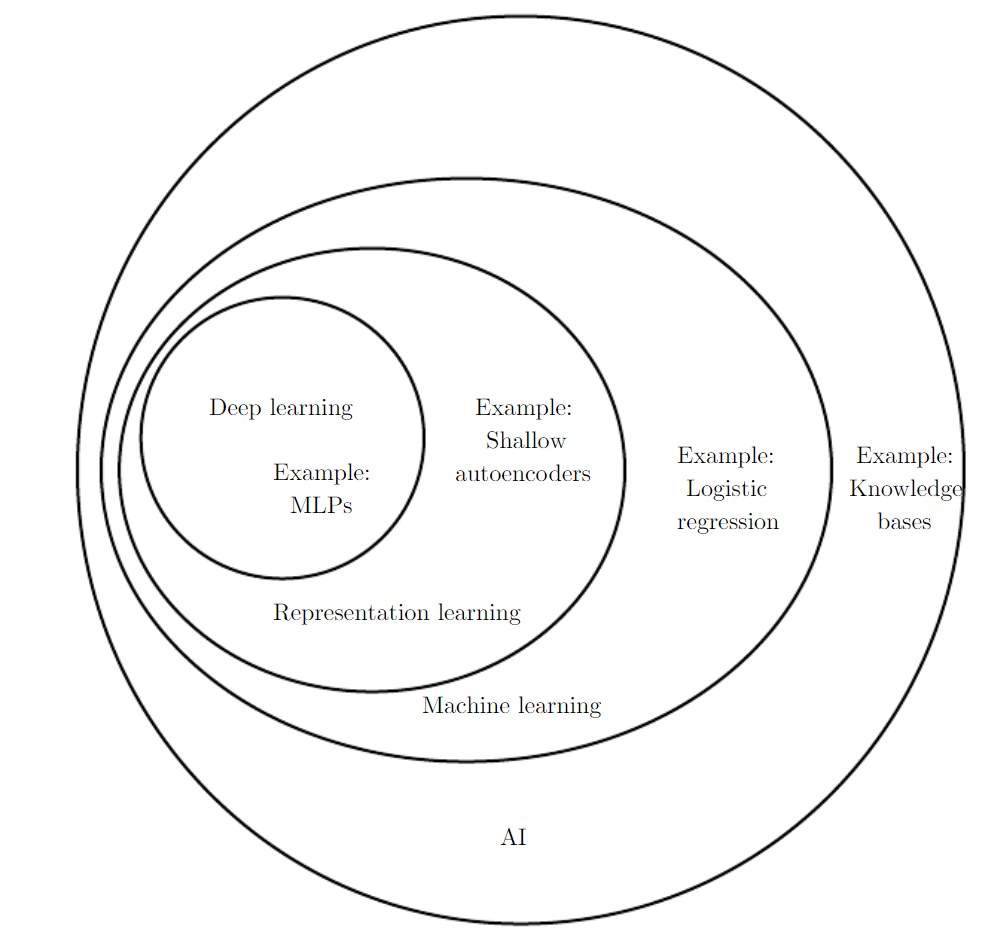
\includegraphics[scale=0.45]{images/venn_diagram_deeplearning.png}
    \centering
    \caption{Biểu đồ Venn về Trí tuệ nhân tạo}
    \label{fig:venn1}
\end{figure}

Một mạng học sâu bao gồm những thành phần sau đây \cite{aws-deep-learning}:
\begin{itemize}
    \item \textbf{Lớp đầu vào:} Một mạng nơ-ron nhân tạo sẽ có một số nút để nhập dữ liệu đầu vào. Các nút này tạo nên lớp đầu vào của hệ thống.
    \item \textbf{Lớp ẩn:} Lớp đầu vào xử lý và chuyển dữ liệu đến các lớp sâu hơn trong mạng nơ-ron. Các lớp ẩn này xử lý thông tin ở các cấp độ khác nhau, thích ứng với hành vi của mình khi nhận được thông tin mới. Các mạng học sâu có hàng trăm lớp ẩn có thể được dùng để phân tích một vấn đề từ nhiều góc độ khác nhau.
    \item \textbf{Lớp đầu ra:} Lớp đầu ra bao gồm các nút xuất dữ liệu. Các mô hình học sâu xuất ra đáp án "có" hoặc "không" chỉ có hai nút trong lớp đầu ra. Mặt khác, các mô hình xuất ra nhiều đáp án hơn sẽ có nhiều nút hơn. 
\end{itemize}

Một điểm đáng chú ý là học sâu cần một lượng lớn dữ liệu để huấn luyện mô hình một cách hiệu quả \cite{wiki-deep-learning}. Trong trường hợp OCR và nhận dạng hóa đơn, mạng nơron học sâu có khả năng học từ hàng nghìn hoặc thậm chí hàng triệu hình ảnh hóa đơn, điều này giúp mô hình hiểu rõ các đặc trưng và biểu diễn của dữ liệu hơn.

Hiện nay các kiến trúc học sâu như mạng nơ-ron sâu, mạng niềm tin sâu, học tăng cường sâu, mạng nơ-ron tái phát, mạng nơ-ron tích chập và máy biến áp đã được áp dụng cho các lĩnh vực bao gồm thị giác máy tính, nhận dạng giọng nói, xử lý ngôn ngữ tự nhiên, dịch máy, tin sinh học, thiết kế thuốc, Phân tích hình ảnh y tế, khoa học khí hậu, kiểm tra vật liệu và các chương trình trò chơi trên bàn cờ, nơi chúng đã tạo ra kết quả tương đương và trong một số trường hợp vượt qua hiệu suất chuyên gia của con người.

\begin{figure}
    \begin{tikzpicture}[x=2.2cm,y=1.4cm]
        \message{^^JNeural network with arrows}
        \readlist\Nnod{4,5,5,5,3} % array of number of nodes per layer
        
        \message{^^J  Layer}
        \foreachitem \N \in \Nnod{ % loop over layers
        \edef\lay{\Ncnt} % alias of index of current layer
        \message{\lay,}
        \pgfmathsetmacro\prev{int(\Ncnt-1)} % number of previous layer
        \foreach \i [evaluate={\y=\N/2-\i; \x=\lay; \n=\nstyle;}] in {1,...,\N}{ % loop over nodes
            
            % NODES
            \node[node \n] (N\lay-\i) at (\x,\y) {$a_\i^{(\prev)}$};
            %\node[circle,inner sep=2] (N\lay-\i') at (\x-0.15,\y) {}; % shifted node
            %\draw[node] (N\lay-\i) circle (\R);
            
            % CONNECTIONS
            \ifnum\lay>1 % connect to previous layer
            \foreach \j in {1,...,\Nnod[\prev]}{ % loop over nodes in previous layer
                \draw[connect arrow] (N\prev-\j) -- (N\lay-\i); % connect arrows directly
                %\draw[connect arrow] (N\prev-\j) -- (N\lay-\i'); % connect arrows to shifted node
            }
            \fi % else: nothing to connect first layer
            
        }
        
        }
        
        % LABELS
        \node[above=5,align=center,mygreen!60!black] at (N1-1.90) {Lớp đầu vào};
        \node[above=2,align=center,myblue!60!black] at (N3-1.90) {Lớp ẩn};
        \node[above=8,align=center,myred!60!black] at (N\Nnodlen-1.90) {Lớp đầu ra};
        
    \end{tikzpicture}
    \centering
    \caption{Kiến trúc một mạng Nơ-ron}

\end{figure}


\subsection{Nguyên tắc hoạt động của OCR}
\subsubsection{Phát hiện văn bản}
\paragraph{DBNet}
\paragraph{SAST}
\subsubsection{Nhận dạng văn bản}
\subsubsection{Trích xuất thông tin chính}